\section*{Experiment 2}

For a single value of the inverting input voltage, we then swept the noninverting input around the inverting one while measuring \Vout. We then fit a straight line to the steep portion of the curve in order to determine the differential-mode voltage (\Adm) gain of the circuit. The experimental results, along with the differential mode gain fit to the curve is shown in Figure \ref{fig:exp2p1}.

From the experimental data, we found $A_{dm} \approx 110$


\begin{figure}[H]
\centering
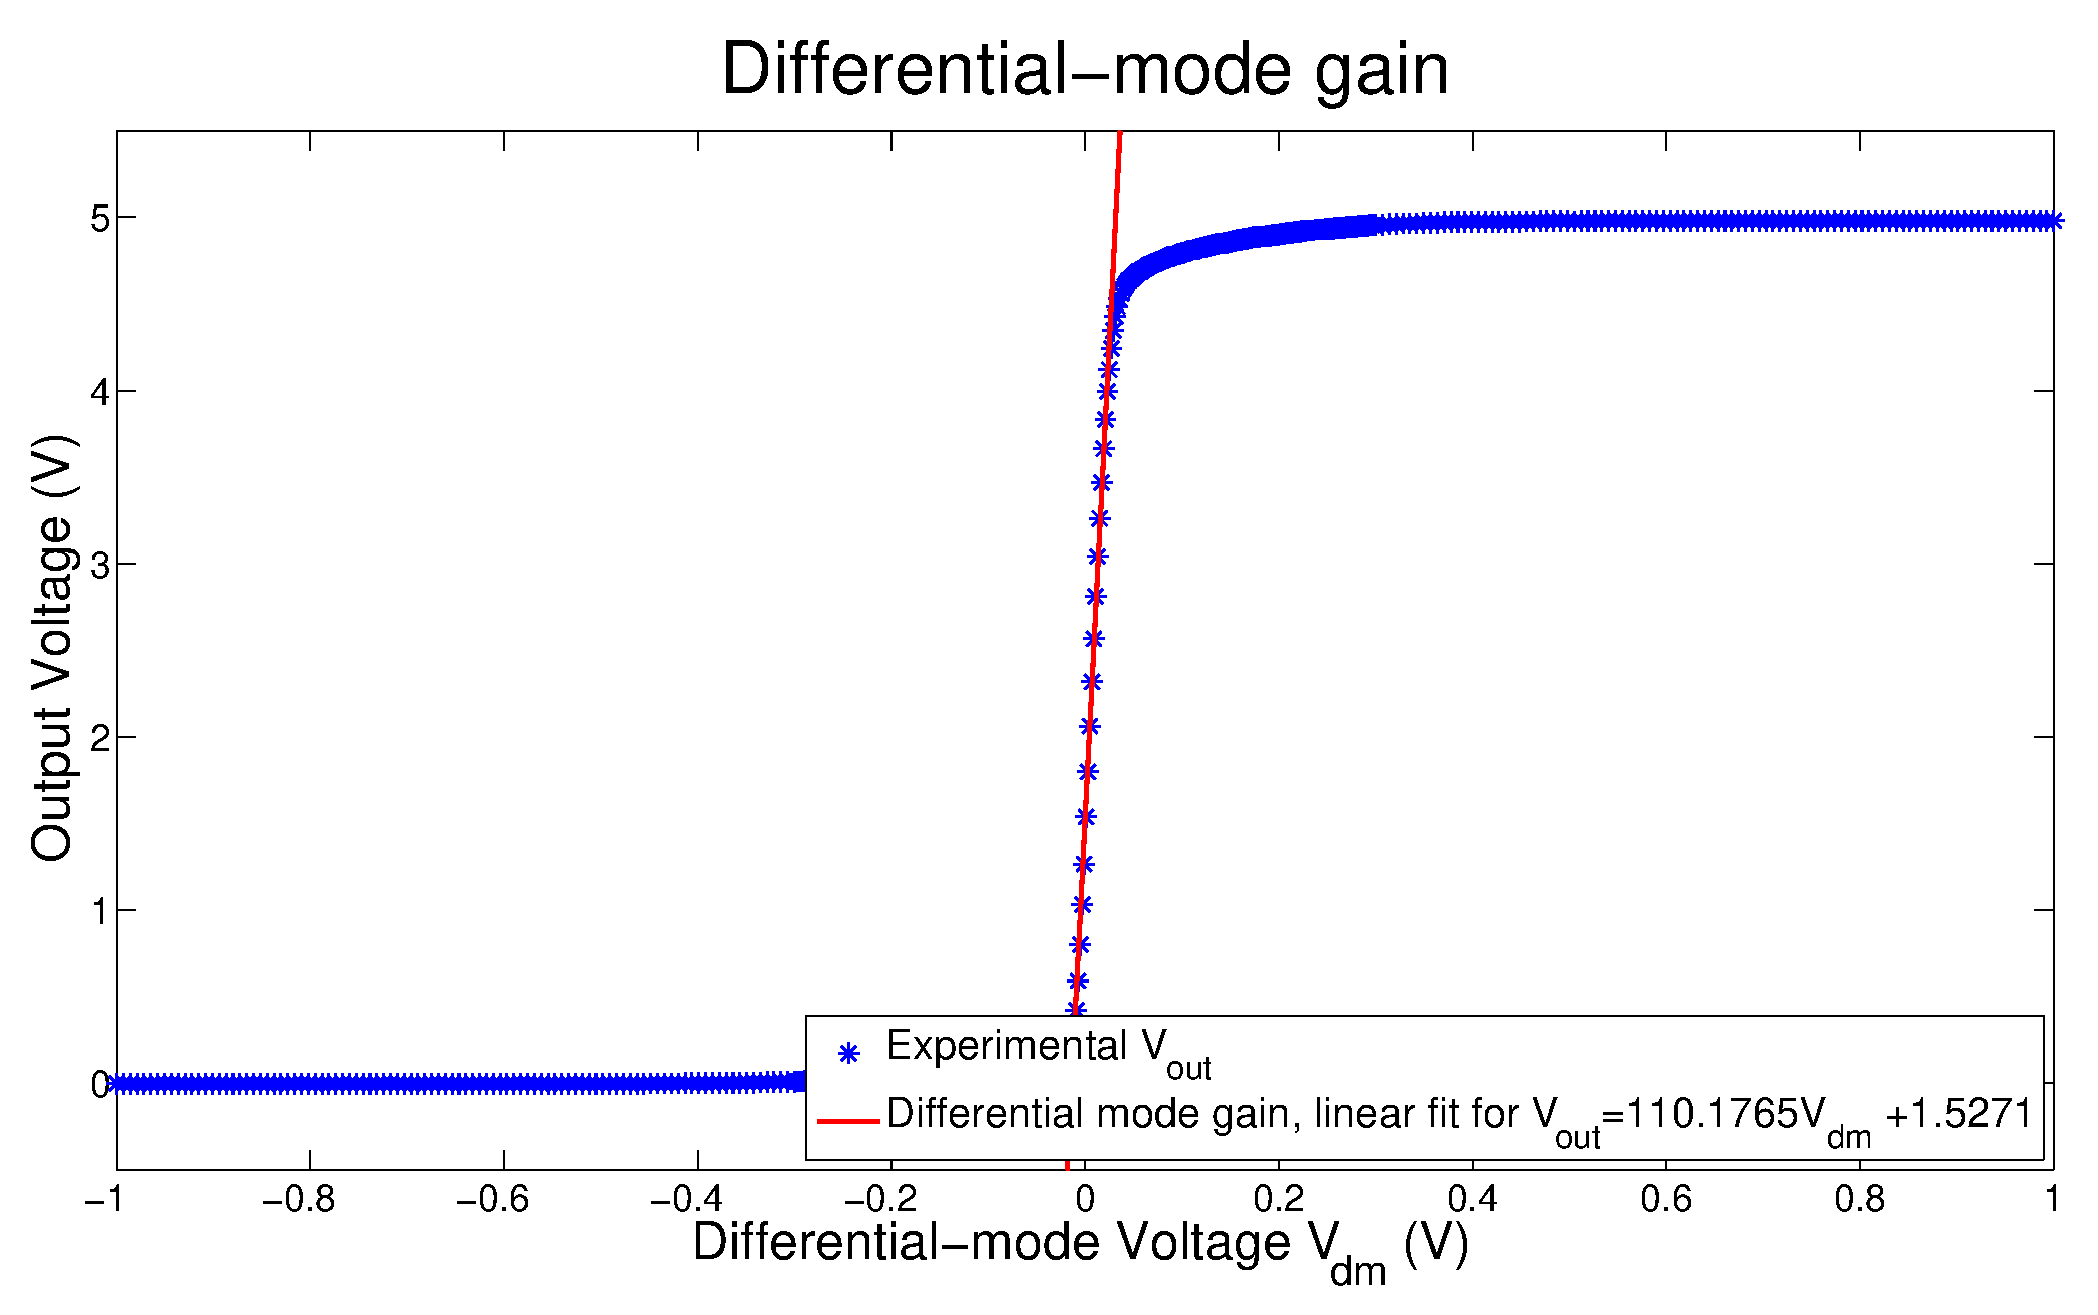
\includegraphics[width=\linewidth]{../Figures/Exp2P1.eps}
\caption{}
\label{fig:exp2p1}
\end{figure}

\begin{figure}[H]
\centering
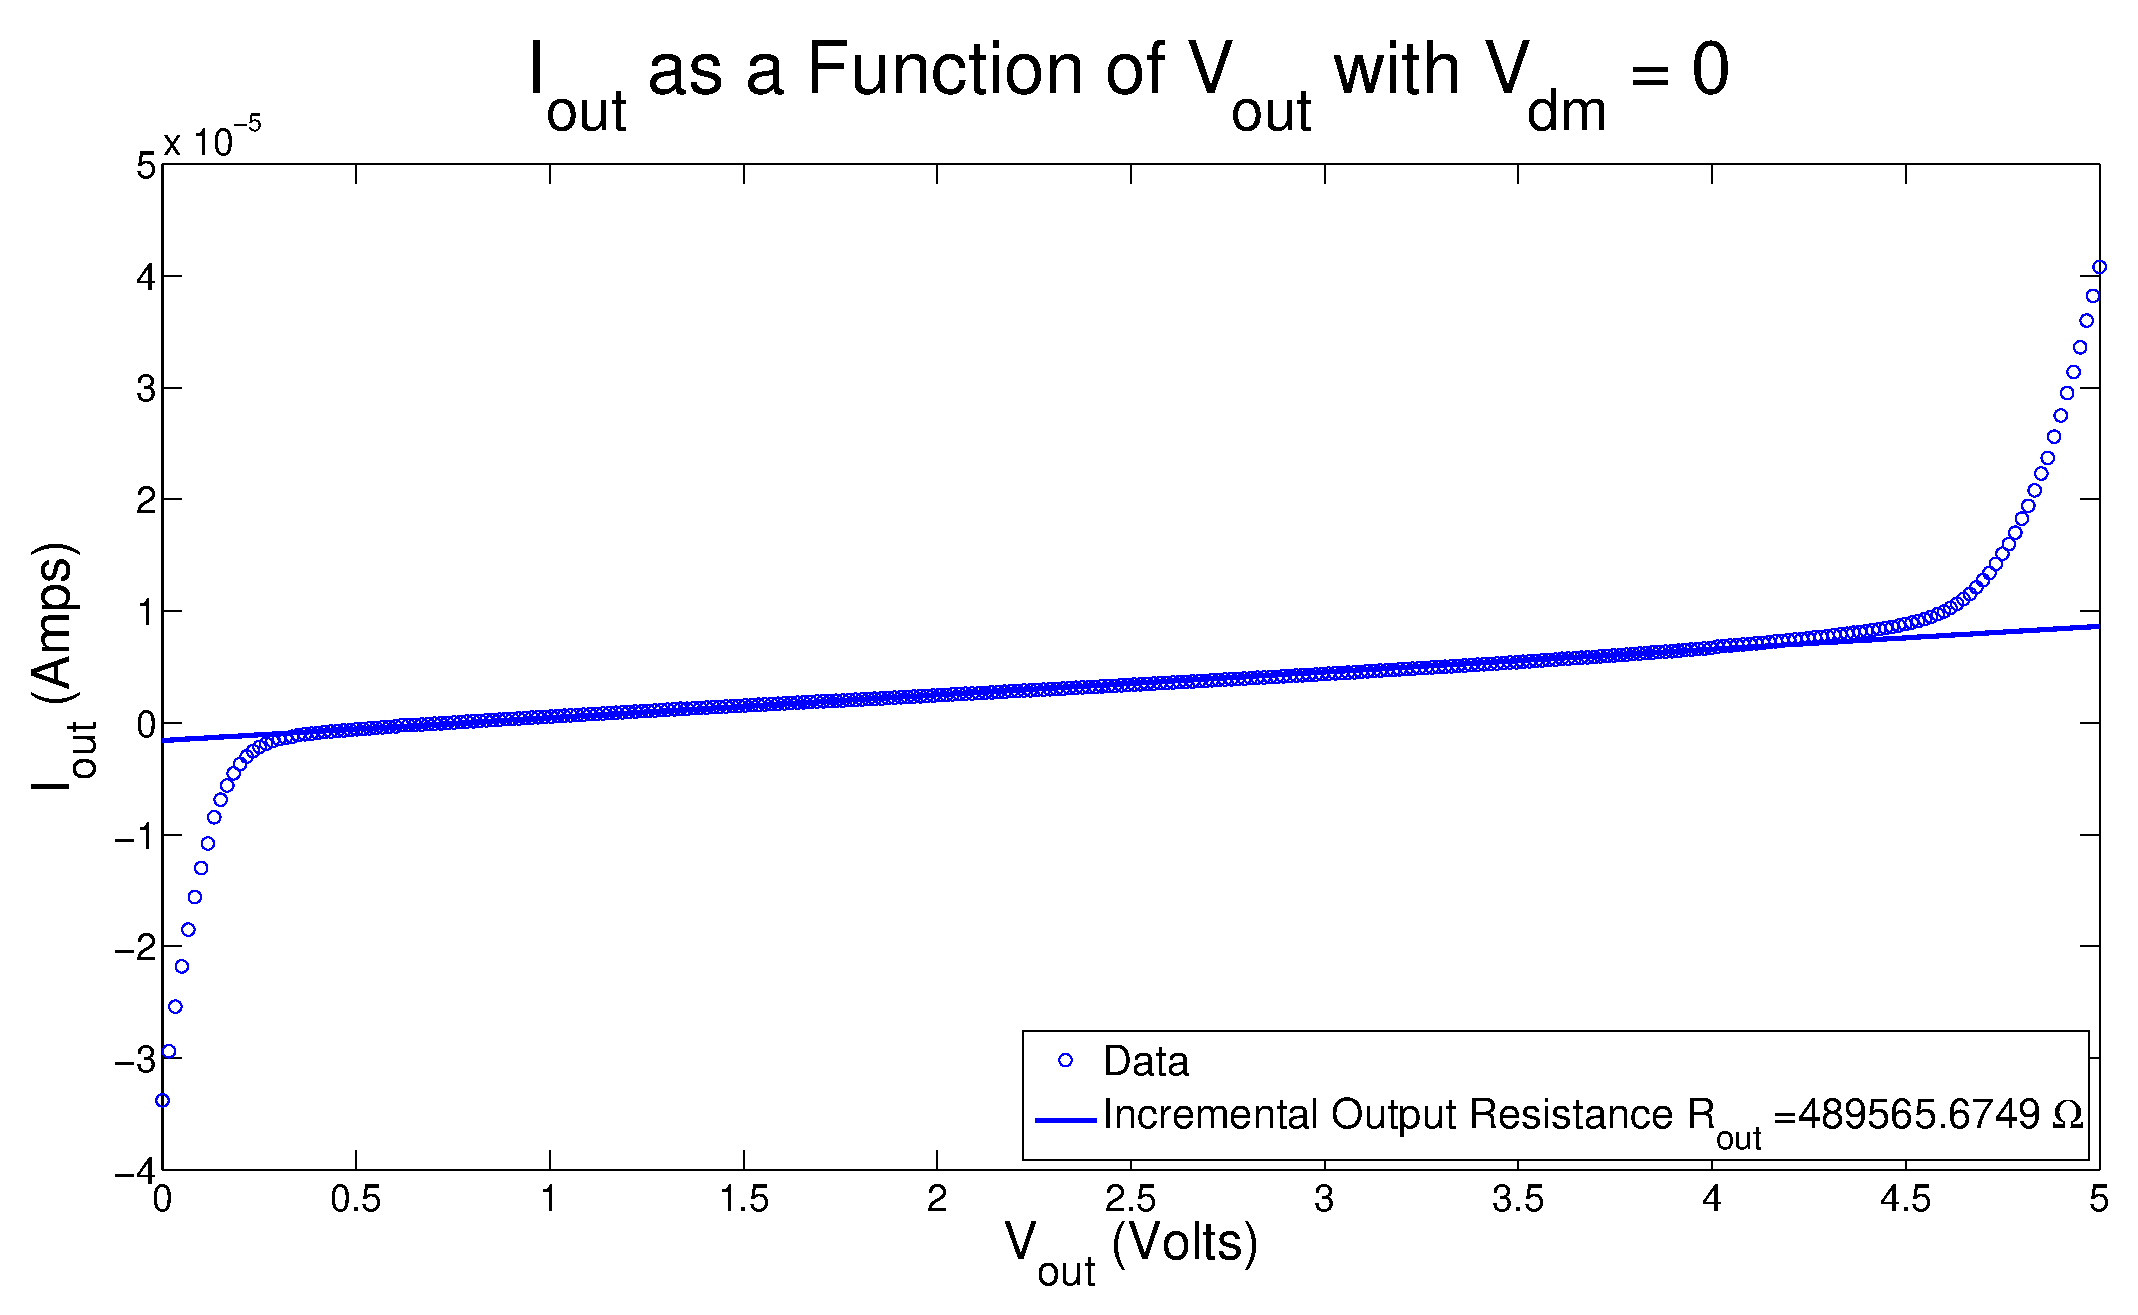
\includegraphics[width=\linewidth]{../Figures/Exp2P2.eps}
\caption{}
\label{fig:exp2p2}
\end{figure}

\begin{figure}[H]
\centering
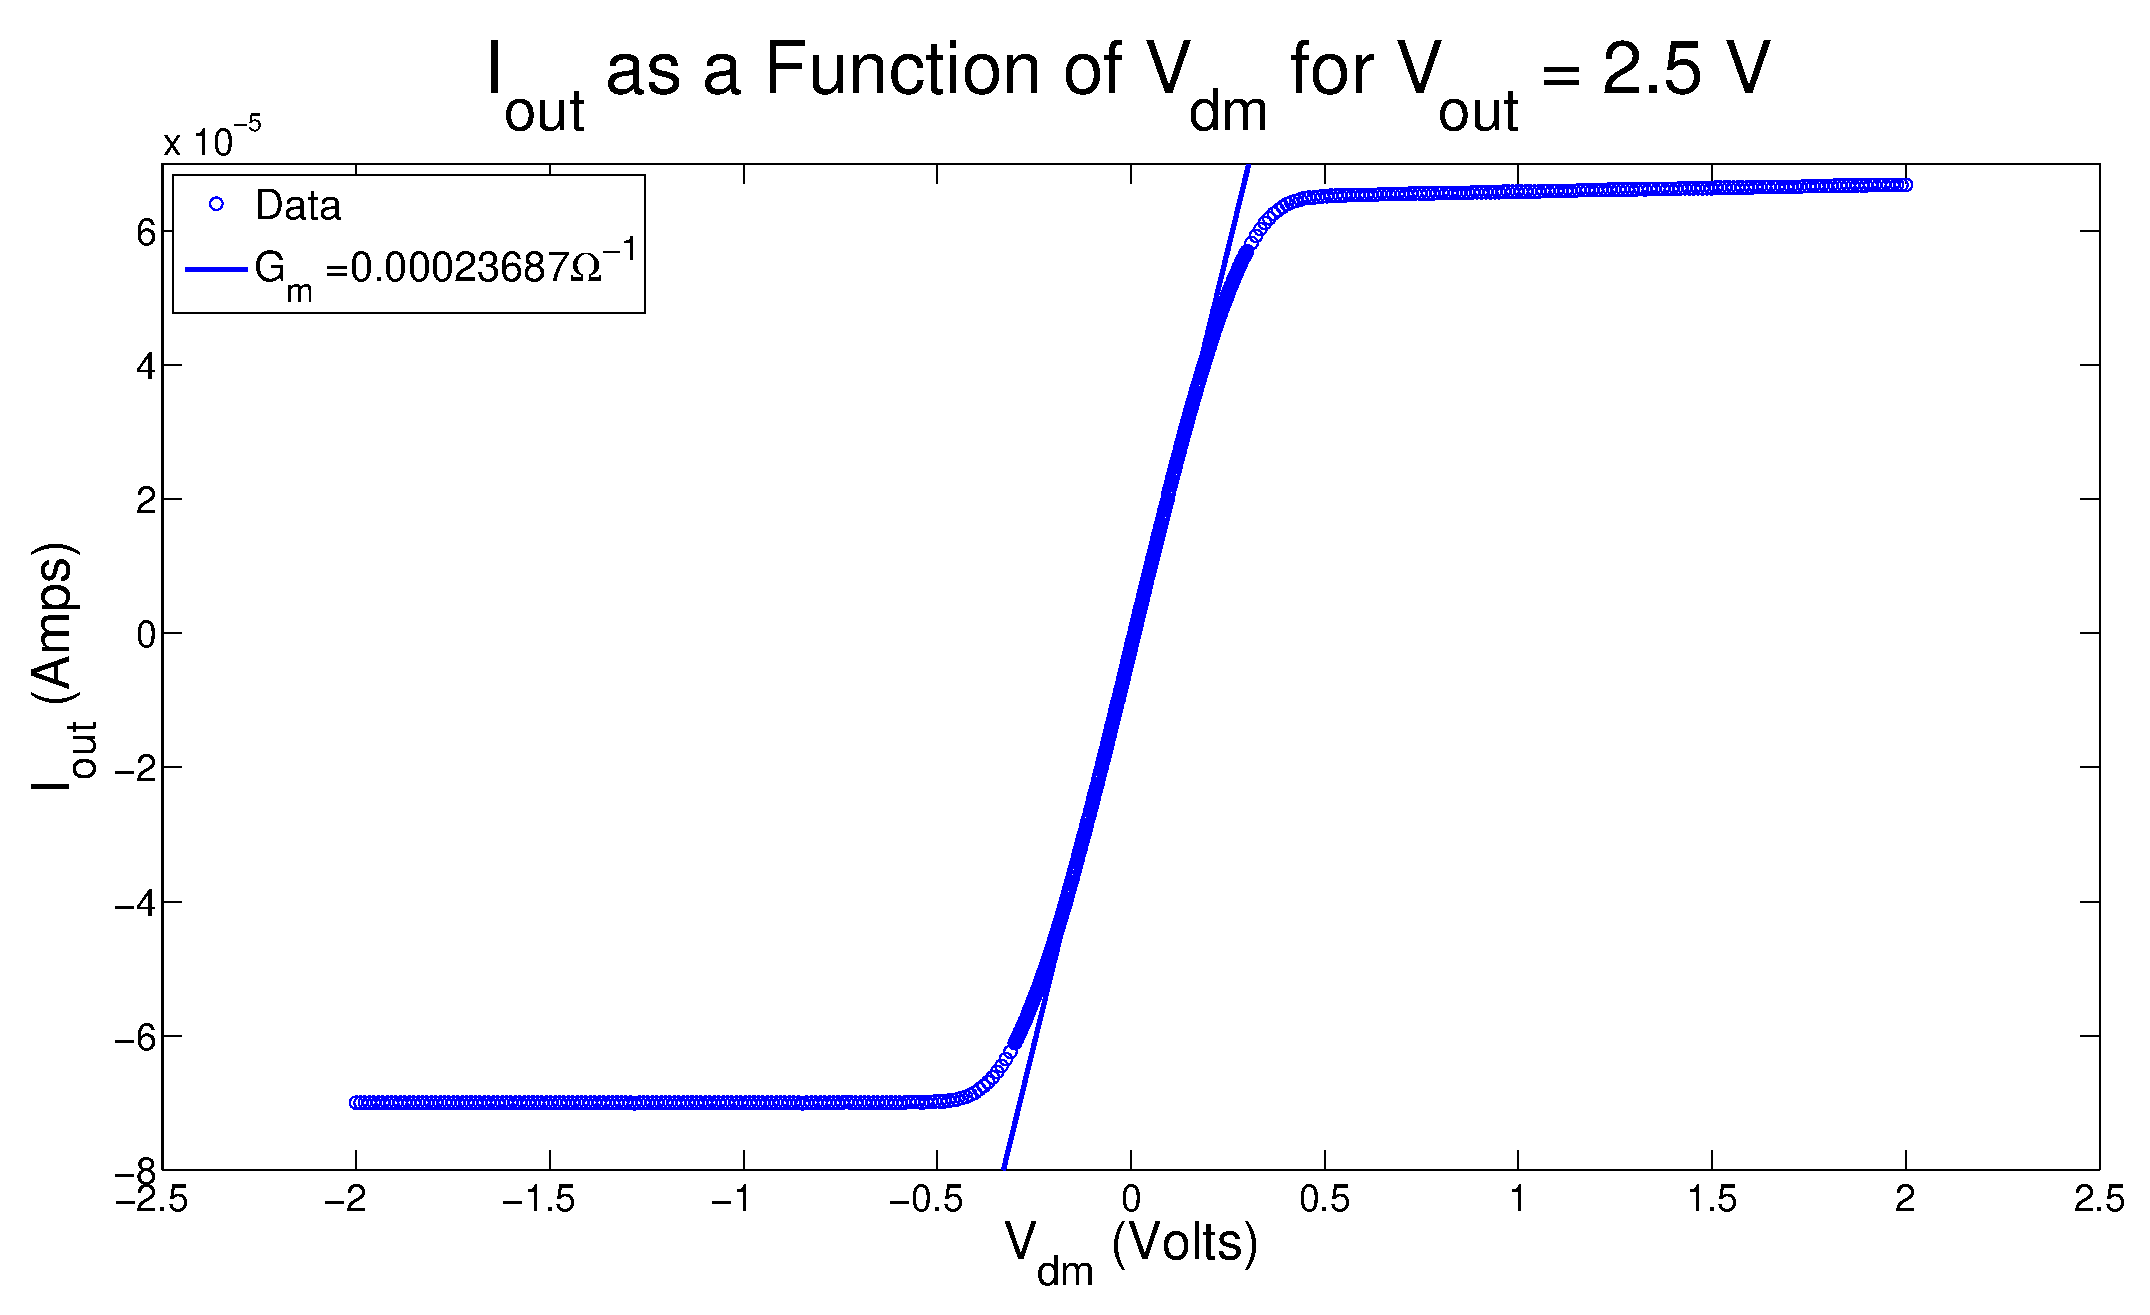
\includegraphics[width=\linewidth]{../Figures/Exp2P3.eps}
\caption{}
\label{fig:exp2p3}
\end{figure}